\PassOptionsToPackage{unicode=true}{hyperref} % options for packages loaded elsewhere
\PassOptionsToPackage{hyphens}{url}
\PassOptionsToPackage{dvipsnames,svgnames*,x11names*}{xcolor}
%
\documentclass[paper=a4,justified,a4paper]{tufte-handout}
\usepackage{lmodern}
\usepackage{amssymb,amsmath}
\usepackage{cleveref}
\usepackage{ifxetex,ifluatex}
\usepackage{fixltx2e} % provides \textsubscript
\ifnum 0\ifxetex 1\fi\ifluatex 1\fi=0 % if pdftex
  \usepackage[T1]{fontenc}
  \usepackage[utf8]{inputenc}
  \usepackage{textcomp} % provides euro and other symbols
\else % if luatex or xelatex
  \usepackage{unicode-math}
  \defaultfontfeatures{Ligatures=TeX,Scale=MatchLowercase}
\fi
% use upquote if available, for straight quotes in verbatim environments
\IfFileExists{upquote.sty}{\usepackage{upquote}}{}
% use microtype if available
\IfFileExists{microtype.sty}{%
\usepackage[]{microtype}
\UseMicrotypeSet[protrusion]{basicmath} % disable protrusion for tt fonts
}{}
\IfFileExists{parskip.sty}{%
\usepackage{parskip}
}{% else
\setlength{\parindent}{0pt}
\setlength{\parskip}{6pt plus 2pt minus 1pt}
}
\usepackage{xcolor}
\usepackage{hyperref}
\hypersetup{
            pdftitle={Assignment 9 - Video Re-recording},
            pdfauthor={Helena Rasche},
            colorlinks=true,
            linkcolor=Maroon,
            filecolor=Maroon,
            citecolor=Blue,
            urlcolor=Blue,
            breaklinks=true}
\urlstyle{same}  % don't use monospace font for urls
\usepackage{graphicx,grffile}
\makeatletter
\def\maxwidth{\ifdim\Gin@nat@width>\linewidth\linewidth\else\Gin@nat@width\fi}
\def\maxheight{\ifdim\Gin@nat@height>\textheight\textheight\else\Gin@nat@height\fi}
\makeatother
% Scale images if necessary, so that they will not overflow the page
% margins by default, and it is still possible to overwrite the defaults
% using explicit options in \includegraphics[width, height, ...]{}
\setkeys{Gin}{width=\maxwidth,height=\maxheight,keepaspectratio}
\setlength{\emergencystretch}{3em}  % prevent overfull lines
\providecommand{\tightlist}{%
  \setlength{\itemsep}{0pt}\setlength{\parskip}{0pt}}
\setcounter{secnumdepth}{0}
% Redefines (sub)paragraphs to behave more like sections
\ifx\paragraph\undefined\else
\let\oldparagraph\paragraph
\renewcommand{\paragraph}[1]{\oldparagraph{#1}\mbox{}}
\fi
\ifx\subparagraph\undefined\else
\let\oldsubparagraph\subparagraph
\renewcommand{\subparagraph}[1]{\oldsubparagraph{#1}\mbox{}}
\fi

% set default figure placement to htbp
\makeatletter
\def\fps@figure{htbp}
\makeatother

\usepackage{pdfpages}

%%%%%%%%%%% Header and Footer %%%%%%%%%%%%%%%%%%
\fancyfoot[CE,CO]{\flushright 
\includegraphics[width=3cm]{../avans.jpg}}
\fancyhead[CE,CO]{\flushleft \smallcaps{\today}}

\usepackage[most]{tcolorbox}
\definecolor{linequote}{RGB}{224,215,188}
\definecolor{backquote}{RGB}{249,245,233}
\newtcolorbox{myquote}{%
    enhanced, breakable,
    size=fbox,
    frame hidden, boxrule=0pt,
    sharp corners,
    colback=backquote,
    borderline horizontal={.5pt}{0pt}{linequote},
    borderline horizontal={.5pt}{1pt}{linequote}
}

\usepackage[]{natbib}
\bibliographystyle{plainnat}

\title[A9 - Video Re-recording]{Assignment 9 - Video Re-recording}
\author{Helena Rasche}
\date{2022-05-11}

\begin{document}
\maketitle
\noindent\rule{5in}{0.4pt}


I hereby submit an updated version of A9. First is the body of the
report, followed by a response to a specific piece of feedback, which I
felt was important to address. However firstly I wish to address:

\begin{myquote}
Asessor 1: Wherever I look in the recording, there is no interaction whatsoever.
Students might as well not exist in this lesson.
\end{myquote}

I worry that this assessor has potentially missed the breakout rooms
which are unfortunately invisible in these videos. I think if it had
been a traditional classroom, I might not have received this comment, as
there \emph{is} significant interaction, but it's not necessarily
present on video.

Please consider that in the intentionally lengthy breakout rooms,
students are taking 20-30 minute periods to

\begin{itemize}
\tightlist
\item
  work together to solve challenging problems
\item
  collaborate and discuss
\item
  determine and implement solutions
\item
  teaching each other, when one is stronger, and learning from the other
  student(s) when they are weaker in this area
\end{itemize}

Here we have a significant amount of student interaction. Additionally I
am often ``walking'' around the breakout rooms to check in on students,
discuss, and answer their questions. All activities which are invisible
on the recording, to the assessor. However since I unfortunately missed
to make separate additional recordings of my time in the breakout rooms
and splice those in with video editing software, this was not present in
the final product for a review that might be skipping through the lesson
observing a minute here and a minute there.

Additionally to further address assessor concerns, I've added a kahoot
at the start to recap the last lesson, and homework question period, and
did a Microsoft Form in chat to determine how long their homework took.

\hypertarget{intervention-fastcups}{%
\section{Intervention: FastCups}\label{intervention-fastcups}}

Per feedback from the assessors who \emph{rightly} point out the lack of
student feedback, I've sought out other methodologies. I absolutely
agree that it is vital to understand how students are feeling about a
topic and if they are successfully keeping up with the material.

To that end, I've introduced the use of
\href{http://cups.fast.ai/}{fastcups}, which mimics a technique I had
previously used in in-person programming classes. There we used post-it
notes (sticky notes), and would have students swap them out based on how
they were feeling. Red for ``I'm struggling!'', yellow for ``I could use
more repetition'', and green for ``It's all good!''

This methodology works exceedingly well, and better than relying on
facial expressions for a significant number of subcases. As an
instructor I am not familiar with all of the variance in cultural
differences of my students, what individual facial expressions mean for
one student may mean a completely different thing for another, based on
background, or, nothing at all. Additionally neurotypical (NT) and
neurodivergent
(ND)\footnote{Here I mostly focus on neurodivergencies like ADHD and ASD which are both co-morbid, and often seems to be present in computer science education, given the author's experiences.}
students may have a different appearance when focusing, ND students may
sometimes look off into nowhere while listening hard, to avoid
distraction. To an NT teacher this looks like being ignored and can lead
to negative interactions and ableism \citep{Clouder2020-ux}. Thus having
a more direct measure of their feelings is important, if I cannot
determine their feelings from visual appearance
alone\footnote{This issue is discussed further in the feedback section.}.

Thus letting students self report their feelings of the class provides
significantly better data than making a guess based off of their
appearance!

\hypertarget{effects-on-students}{%
\section{Effects on students}\label{effects-on-students}}

Students were much more able to communicate their feelings back to me as
a teacher, and the addition of the anonymity allows them to be more
honest in their reviewing{[}10.1016/j.jesp.2014.07.014{]}. When the
teacher view of the tool was on screen, students could see the responses
of their classmates (in aggregate) and feel more comfortable in not
being the only person feeling behind or needing more explanation.

As a teacher I was really pleased with the effect of the tool; I could

\begin{enumerate}
\def\labelenumi{\arabic{enumi}.}
\tightlist
\item
  Ask students ``please update fast cups, how do you feel?''
\item
  See the result trend towards yellow and red
\item
  Then slow down and re-explain the topic
\item
  Ask again
\item
  And see more green.
\end{enumerate}

This really quick interaction turnaround time produced a more efficient
classroom (e.g.~timepoints 39:00 - 41:38 / 2:23:55 - 2:29:18) I'm not
waiting for students to unmute and respond in front of their classmates,
they're able to tell me instantaneously, with no loss of privacy. And
for me as a teacher, that instantaneous feedback is invaluable,
especially since it is provided in a way that does not disrupt the flow
of the lesson.

\hypertarget{lessons-learned}{%
\section{Lessons Learned}\label{lessons-learned}}

If I am to continue in my preferred modality, and even if not (given
inability to read faces with any accuracy, as a new teacher), I should
absolutely be employing this tool consistently throughout my classes to
get feedback from students on how they are experiencing the class. I
think this gave students significantly more options for interaction
throughout the lesson in ways that work for them, based on Assignment 8.
Additionally given the context of the type of person attracted towards a
computer science based curriculum and their learning preferences, versus
say the type in a business course, this methodology meshes well with the
students.

\hypertarget{tips-tops-the-future}{%
\section{Tips \& Tops \& the future}\label{tips-tops-the-future}}

Top: Seeing student responses go from yellow and red to green (and some
yellow) following an explanation was a great feeling, and gave me
significant confidence in the methodology, that I could react so quickly
to their feelings. Additionally having the student responses on screen
occasionally, combined with anonymity, perhaps gave them more confidence
in asnwering that they were having difficulties. It is common across
teaching, I believe, for students to feel alone in being slow or behind,
when in fact everyone is, and it only becomes apparent during
discussions.

Tip: During the course I developed a concern for low response rate, that
perhaps students were not actively updating their ``cups'', and in a
future revision I will explore implementing a ``clear'' function, to
allow deleting their responses and then requesting them freshly, to make
sure the majority of students are responding. Additionally I should make
sure that the interface is always visible so I can appear to be more
responsive to it. I was watching my phone with the interface, but, this
may not have been apparent to students.

\hypertarget{feedback}{%
\section{Feedback}\label{feedback}}

I specifically wish to address this feedback, because I worry the
assessor is not up to date on the equity and inclusion issues present

\begin{myquote}
But if you give students the freedom to hide behind a closed camera, it
can have negative consequences for your students and for you. It's not
good for their bonding with you and their peers. And it's not good for
their engagement in class. And it offers you less insight into your
students and therefore less feeling about whether what you do with it,
does land with them.
\end{myquote}

The potentially resulting cyberbullying, racism, and ableism, lead me to
consciously make different choices, which I discuss below. I understand
the reason for the criticism, but disagree with the solution, I think we
can find alternatives that are better.

\hypertarget{hypothetical}{%
\subsection{Hypothetical}\label{hypothetical}}

Consider first the \emph{Gedankenexperiment}: if seeing students is of
such paramount importance, then we should \textbf{immediately} fire
blind and visually impaired teachers, as they cannot be effective as
teachers.

This I think is obviously the wrong answer, and demands that we search
for altenative, inclusive solutions, as blind and visually impaired
teachers can absolutely still be effective\citep{afzal2021sighted}.

\hypertarget{home-invasion}{%
\subsection{Home Invasion}\label{home-invasion}}

Requiring that cameras be on risks intruding into the personal lives of
students' homes (or lack thereof), putting learners education second and
their personal lives front and center, on display for their fellow
students. This risks highlighting disparities between students. Many
students do not have the luxury of a ``blank'' space they can show, and
the constantly visible cameras may be distracting or even voyeuristic
\citep{reed_2020, ng2020communicative} thus intruding into their
personal lives and opening the doors for cyberbullying from their peers.

I personally have a pride flag hanging in one room, this feels like
unnecessary oversharing of my personal life with students. However,
\emph{because} I am \emph{privileged}, and between my partner and I, we
have a flat with multiple rooms, I am able to find a less distracting
and personal background from which to teach.

Virtual backgrounds are a common retort here, but they are inconsistent,
and not available across all platforms. Until recently, Zoom required
chromakeying (a greenscreen, with extra cost) to do virtual backgrounds
on
Linux\footnote{in bioinformatics, many students use Linux instead of Windows or Apple's OSX, as it is more appropriate.},
and teams likewise does not support it on all platforms.

The simplest, most effective solution to this issue, while the ongoing
pandemic forces us online, is to simply not demand it, and seek out
alternative solutions. In the future we'll all be able to return to
classrooms, and this issue will not be present.

\hypertarget{neurodiversity}{%
\subsection{Neurodiversity}\label{neurodiversity}}

Some, neurodiverse students may not learn best while sitting still, and
be distracted by the social pressure to, or may not want classmates to
know they prefer to move around while following the
lecture\citep{duncan2021}.

Anecdotally, in my personal experiences within Bioinformatics (which I
teach) and Computer Science (a closely affiliated discipline), the
incidence rates of neurodiverse peers is significantly higher than in
other fields, as the environments and jobs available often are very
suited to folks whose brains work differently, but just as well as the
rest of us.

\hypertarget{why-wont-they}{%
\subsection{Why won't they?}\label{why-wont-they}}

Students worry actively about things in their home, siblings, pets, or
their appearance being distracting .

\citep{10.1002/ece3.7123} surveyed students and found the following
reasons

\begin{itemize}
\tightlist
\item
  I was concerned about my appearance {[}A, B{]}
\item
  I was concerned about other people being seen behind me {[}A{]}
\item
  I was concerned about my physical location being seen behind me {[}A,
  B{]}
\item
  I was concerned about distracting my classmates
\end{itemize}

Where A are things that affect under represented minorities more than
Cis/Het-White-Male students, and B are items that affect female students
more than male students. None of these are desireable feelings that
students should experience, and this concern is easily removed by not
requiring cameras.

\hypertarget{what-can-we-really-tell}{%
\subsection{What can we really tell?}\label{what-can-we-really-tell}}

When even teens are able to subvert the camera \citep{vice} and use
looped videos á la heist movies, the value of obsessing over this is
very suspect. It's not our job to police their behaviour, and even if we
try to, what can we really tell?

\begin{figure}
\centering
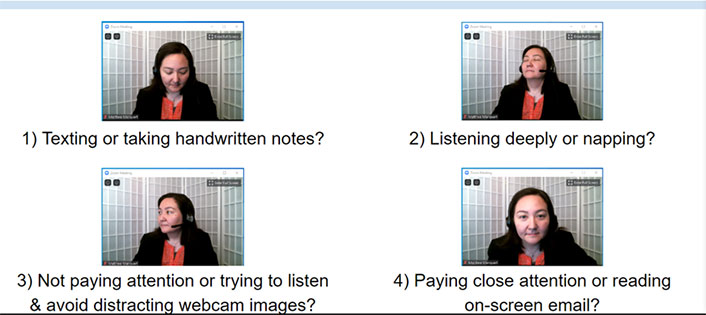
\includegraphics{educase.jpg}
\caption{Example from \citep{educase} highlighting the sheer difficulty
in reading a student's body language}
\end{figure}

This is not an activity I wish to dedicate my time to, discering the
body language of students and making uneducated guesses at what their
behaviour represents. I'd love for them to pay attention, but they are
adults, they will make their own choices.

\hypertarget{sec:report}{%
\section{Classroom Management}\label{sec:report}}

Overall the classroom is fine, I have essentially zero issues with
misbehaviour or disruptive behaviour. They're all adults by this point
in their career, they know what's expected of them, and they're starting
to understand the independence that's expected of them in the workplace.
What really works for me is treating them like adults and holding them
to the same standards I'm held to in meetings I attend; if I want my
camera off it stays off, if my back-to-back meetings mean I need to eat
then I do with mic and camera off. Additionally it is important to note
that this classroom is a \emph{subset} of the interactions I have with
these students, but by only submitting the classroom recording as
evidence, a very limited picture is given of relationships with students
and out of class interactions. I am regularly in communication with them
via email, teams, and other meetings which provide for different
interaction modalities.

\bibliography{report.bib}

\end{document}
